\question %5
\emph{Testez sous MATLAB la procédure du point précédent avec les données
fournies. Comparez ensuite la prédiction obtenue par cette procédure
avec la valeur obtenue en résolvant à nouveau complètement le modèle,
et ce pour un échantillon de valeurs du paramètre \texttt{epsilon} comprises
entre $0$ et $1$ (par exemple \texttt{0:.1:1}). 
Commentez (éventuellement en vous aidant d'un graphique).}

Comparaison À FAIRE.

Notre fonction \texttt{compareDuality.m} permet de prouver l'efficacité
du problème dual lorsqu'on perturbe le vecteur des contraintes.
En effet, si l'on décide d'analyser via le problème primal ce qu'il 
se passe lorsque les contraintes sont modifiées, il est nécessaire de 
résoudre le problème à chaque perturbation 
(plusieurs appels à \texttt{linprog}).
Tandis que pour le problème dual,
il suffit d'effectuer plusieurs combinaisons linéaires de la fonction objectif
avec \emph{une seule} solution $y^{*}$ 
(c'est-à-dire un apppel à \texttt{linprog}).
On retrouve les résultats des tests d'efficacité
sur le graphe de la figure~\ref{fig:efficiencyDual}. 

Cependant, comme expliqué dans la section précédente, ce résultat n'est valable que pour des petites variations des contraintes.
Si \texttt{epsilon} devient trop grand, l'analyse par le primal pourrait diverger de la solution du primal.
C'est ce que nous obtenons en implémentant ces deux méthodes, comme représenté à la figure \ref{fig:responseToPerturbations}

\begin{figure}
  \begin{center}
    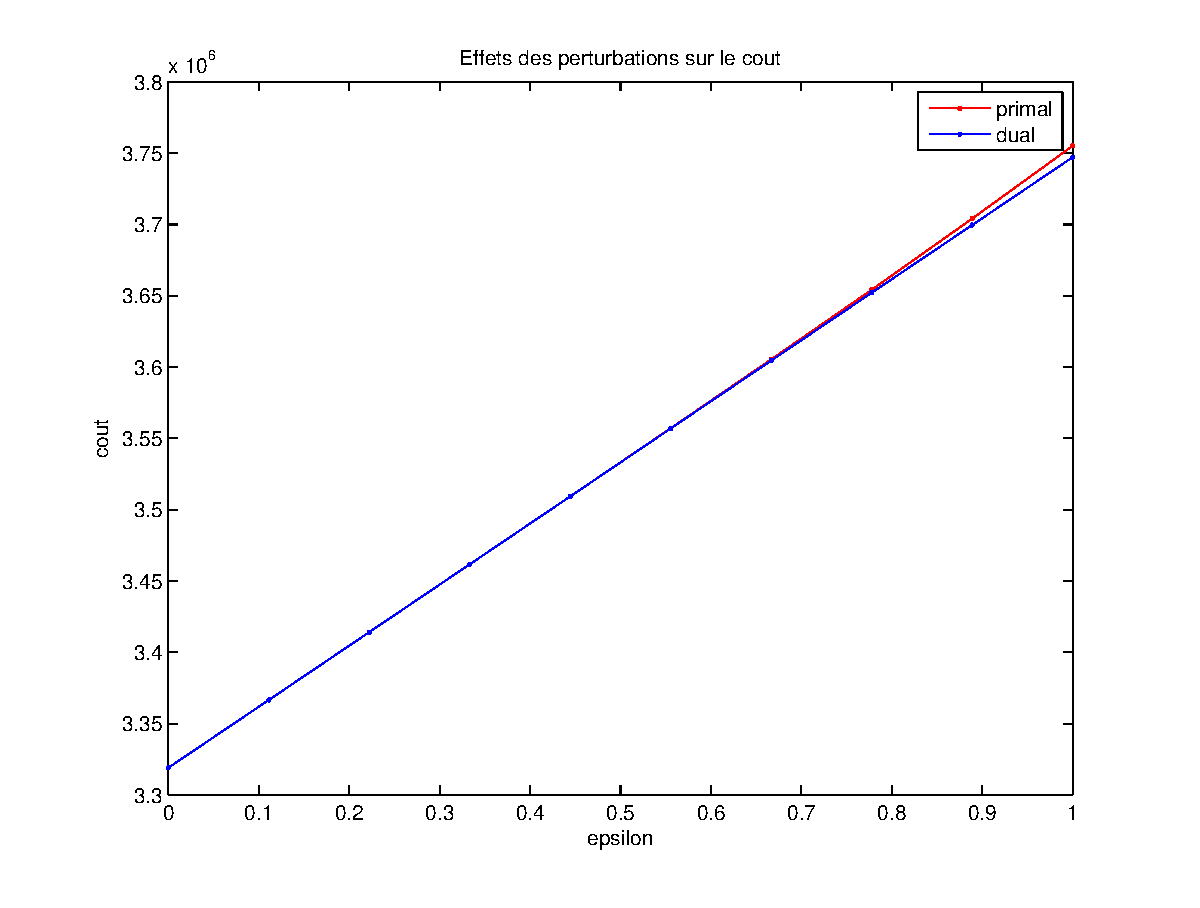
\includegraphics[scale=0.6]{img/responseToPerturbations.eps}
    \caption{Comparaison de la réponse aux perturbations du primal 
    et dual. On remarque que les valeurs restent égales jusqu'à 
    $\epsilon \approx 0.6$.}
    \label{fig:responseToPerturbations}
  \end{center}
\end{figure}

\begin{figure}
  \begin{center}
    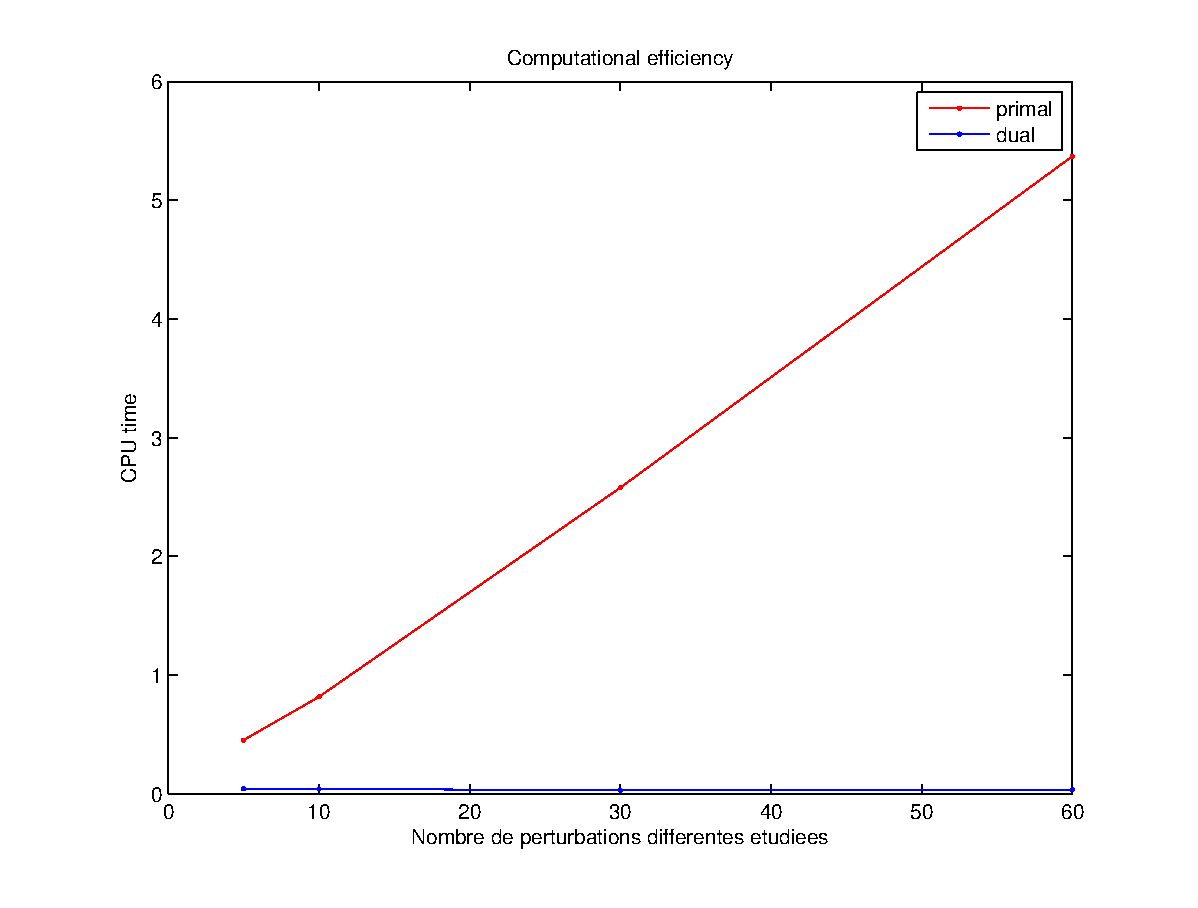
\includegraphics[scale=0.6]{img/efficiencyDual.eps}
    \caption{Comparaison de l'efficacité du primal et dual lors de
    l'analyse de perturbations sur les contraintes.}
    \label{fig:efficiencyDual}
  \end{center}
\end{figure}
